\section{Methods}
\label{sec:methods}

In this section, we present the methods used to solve the problem of learning nonlinear deformation modes. We provide a brief overview of the theoretical background of neural networks, then explain the idea behind subspace learning. \textcolor{blue}{hai scritto al contrario le due subsection}

\textcolor{blue}{non ho capito cosa centra il subspace learning}

\textcolor{blue}{non hai nominato le cose che fai dopo (3.3, 3.4)}

\subsection{Subspace Learning}

Let \( \bm{X} \in \mathbb{R}^{n \times d} \) and \( \bm{x} \in \mathbb{R}^{d} \) be the vectors representing the undeformed and deformed configurations of a mesh, respectively. We can characterize equilibrium configurations of the system by constrained energy minimization principles \textcolor{blue}{secondo me puoi spiegarlo meglio io non ho capito}, such as 
\begin{align*}
    \bm{x}^*(\phi, \psi) = \underset{\bm{x}}{\argmin} \quad & E_\phi(\bm{x}) \\
    \text{s.t.} \quad & C_\psi(\bm{x}) = 0,
\end{align*}
where \( E_\phi \) is the energy function defined by parameters \(\phi\) and \( C_\psi \) is the constraint function with parameters \(\psi\). The solution set \( \bm{x}^*\) constitutes a subspace of the full-dimensional space \( \mathbb{R}^d \). In a classical Finite Element framework, sampling from this subspace is achieved by solving a constrained minimization problem for each configuration. 

Clearly, this approach is computationally expensive, so we need a more efficient way to sample from the subspace.

The idea proposed by \cite{Wang_Du_Coros_Thomaszewski_2024} is to find a Neural Network \( \bm{x}[\theta^*](\phi, \psi) \) that approximates the solution \( \bm{x}^* \), meaning that the problem becomes:
\begin{align*}
    \bm{x}[\theta^*](\phi, \psi) \approx \underset{\theta}{\argmin} \quad & E_\phi(\bm{x}[\theta](\phi, \psi)) \\
    \text{s.t.} \quad & C_\psi(\bm{x}[\theta](\phi, \psi)) = 0.
\end{align*}

Now, defining the nonlinear modes as 
\begin{align}
    \bm{n}(\bm{z}) = \bm{l} + \argmin_{\bm{y}} \quad & E_\phi(\bm{X} + \bm{l} + \bm{y}) \\ 
    \text{s.t.} \quad & \bm{l}^T \bm{y} = 0,
\end{align}
where \( \bm{l} \) is the linear mode displacement obtained as
\begin{equation}
    \bm{l} = \sum_{i=1}^m z_i \bm{e}_i,
\end{equation}
where \( \bm{e}_i \) is the $i$-th linear mode and \( z_i \) is the corresponding modal coordinate, we can rewrite the problem \textcolor{blue}{quale?} as
\begin{align*}
    \bm{n}[\theta^*](\bm{z}) &= \bm{l} + \bm{y}[\theta^*](\bm{z}), \\
    \theta^* = \underset{\theta}{\argmin} \quad & E_\phi(\bm{X} + \bm{l} + \bm{y}[\theta](\bm{z})) \\
    \text{s.t.} \quad & \bm{l}^T \bm{y}[\theta](\bm{z}) = 0.
\end{align*}

Now we define a suitable function that will serve as a loss function for the self-supervised training of the neural network. The loss function is defined as:
\begin{equation}
    \mathcal{L}(\theta) = \mathbb{E}_{\bm{z}} \left[ E(\bm{X} + \bm{l} + \bm{y}[\theta](\bm{z})) + \lambda_1 \bm{l}^T \bm{y}[\theta](\bm{z}) + \lambda_2 \|\bm{y}[\theta](\bm{z})\|^2 \right],
\end{equation}
where \( \lambda_1 \) and \( \lambda_2 \) are hyperparameters that control the importance of the orthogonality and origin loss terms, respectively\textcolor{blue}{ the importance?}. The first term is the energy loss, which minimizes the internal strain energy of the deformed configuration, while the second term ensures that the nonlinear correction is orthogonal to the linear mode space. The third term is \textcolor{blue}{an expression} that ensures that the neural network is centered at the origin.


\subsection{Neural Network Basics \textcolor{blue}{Principles?}}

A Neural Network (NN) is a mathematical model that achieves statistical generalization drawing inspiration from the human brain. \textcolor{blue}{Indeed, it is based on neurons, which are connected one to another, and carry the information from the input to the output.} 

It is possible to define NN as a function that maps an input to an output, given a set of parameters \( \bm{\theta} \). The function \( \hat{y} = f(\bm{x}; \bm{\theta}) \) is obtained by composing a series of functions \( f_i \) called layers, where each layer is defined as
\begin{equation}
    f_i = \sigma(W_i f_{i-1} + b_i),
\end{equation}
where \( W_i \) is the weight matrix, \( b_i \) is the bias vector and \( \sigma(\cdot) \) is the activation function. The activation function is a non-linear function that allows the network to learn complex patterns in the data. 

A neural network exists in function of a dataset \( \mathcal{D} = \{(\bm{x}_i, \bm{y}_i)\}_{i=1}^N \), where \( \bm{x}_i \) is the input and \( \bm{y}_i \) is the output. The final goal is to find the set of parameters \( \bm{\theta} \) that minimizes the loss function \( \mathcal{L} \), defined as some metric of the difference between the predicted output and the true output. The loss function:
\begin{equation}
    \mathcal{L} = \frac{1}{N} \sum_{i=1}^N L(f(\bm{x}_i; \bm{\theta}), \bm{y}_i)
\end{equation}
where \( L \) is the loss function, which can be various metrics. The loss function is minimized using an optimization algorithm, so that the objective is to find
\begin{equation}
    \bm{\theta}^* = \argmin_{\bm{\theta}} \mathcal{L}
\end{equation}
which is the best set of parameters that minimizes the loss function. \textcolor{blue}{hai chiamato loss function sia quella dentro che quella fuori, non si capisce molto}

The full algorithm is the following one:
\begin{algorithm} 
    \caption{Training of a neural network}
    \begin{algorithmic}
        \State Initialize the parameters \( \bm{\theta} \)
        \While{epoch < max\_epochs}
            \For{mini-batch in dataset}
                \State Perform forward pass computing \( f(\bm{x}; \bm{\theta}) \)
                \State Compute the loss function \( \mathcal{L}(f(\bm{x}; \bm{\theta}), \bm{y}) \)
                \State Perform backward pass computing the gradients of the loss function
                \State Update the parameters using the gradients
            \EndFor
        \EndWhile
    \end{algorithmic}
\end{algorithm}

\textcolor{blue}{Ho un intero paragrafo sulle nn, se serve allungare}

\subsection{Neural Network Architectures}
In this work, we employ a deep feedforward neural network specifically designed for learning nonlinear deformation modes. This architecture builds upon traditional fully connected neural networks but is adapted for the specific task of capturing nonlinear corrections to linear modal displacements.

\subsubsection{Neural Modes Architecture}
The Neural Modes architecture is designed to learn nonlinear corrections to linear deformation modes for Neo-Hookean materials. It consists of a Feed-Forward Neural Network (FFNN)\textcolor{blue}{, a type of artificial neural network where the connections between the nodes do not form cycles,} where:

\begin{itemize}
    \item The input is a modal coordinate vector \( \bm{z} \in \mathbb{R}^m \), where $m$ is the number of modal coordinates.
    \item The output is a nonlinear correction to the displacement field \( \bm{y} \in \mathbb{R}^n \), where $n$ is the total number of degrees of freedom in the mesh.
\end{itemize}

The network learns to map from the reduced modal space to full-dimensional correction vectors that improve the accuracy of the linear modal approximation. This architecture can be visualized as: \textcolor{blue}{io ti direi di allungare qui in giro}
% H per bloccare la figura. altrimenti metti la referenza
\begin{figure}[H] 
    \centering
    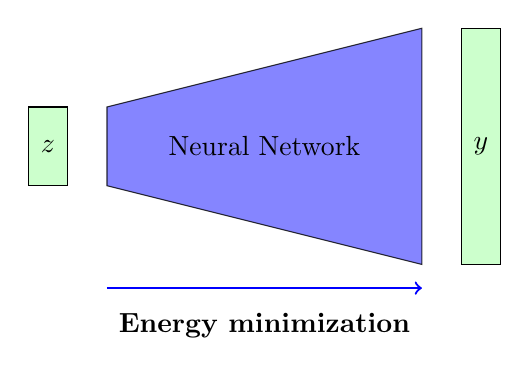
\begin{tikzpicture}
        % Modal coordinate (z)
        \draw[fill=green!20] (-3, 1) rectangle (-2.5,2);
        \node at (-2.75, 1.5) {$\bm{z}$}; % Label inside the rectangle
        
        % Displacement (u)
        \draw[fill=green!20] (2.5,0) rectangle (3,3);
        \node at (2.75, 1.5) {$\bm{y}$}; % Label inside the rectangle
        
        % Energy loss transition
        \draw[fill=blue!60,opacity=0.8] (-2,1) -- (2,-0) -- (2,3) -- (-2,2) -- cycle;
        \node at (0,1.5) {Neural Network};
        \node[below] at (0,-0.5) {\textbf{Energy minimization}};
        
        % Energy loss arrow
        \draw[thick,blue,->] (-2,-0.3) -- (2,-0.3);
    
    \end{tikzpicture}
    \caption{Neural Modes architecture for learning nonlinear deformation corrections}
    \label{fig:neural_modes_arch}
\end{figure}

\subsubsection{Training the Neural Modes}
The training process for the Neural Modes Network is based on minimizing a combination of physics-based losses, rather than simply minimizing the prediction error against ground truth data\textcolor{blue}{, which is the classical loss used in most neural network training}. The key \textcolor{blue}{ terms that build the }loss used in training are:

\begin{enumerate}
    \item \textbf{Energy Loss}: minimizes the internal strain energy of the deformed configuration $E(\bm{X} + \bm{l} + \bm{y})$, where $\bm{X}$ is the rest position, $\bm{l}$ is the linear mode displacement given by $\bm{z}$, and $\bm{y}$ is the nonlinear correction.
    
    \item \textbf{Orthogonality Loss}: ensures that the nonlinear correction is orthogonal to the linear mode space: $\bm{y}^T \bm{l} = 0$.
    
\end{enumerate}

The total loss function is a weighted sum of these individual losses:
\begin{equation}
    \text{Loss} = \text{Energy Loss} + \lambda_1 \text{Orthogonality Loss} + \lambda_2 \text{Origin Loss},
\end{equation}
where $\lambda_1$ and $\lambda_2$ are weight parameters that balance the importance of each loss term.

During the training process, it was observed that the network had the tendency to learn a correction when given \(z = 0\) (i.e., the rest position), and that was not intended, because the rest position should not have any correction, meaning that the model prediction should be zero. To avoid this, the network was designed to have zero bias, so that its output was centered at the origin. \textcolor{blue}{chi lo osserva, quando come perchè? quindi si aggiunge il terzo termine che prima non nomini? allora metti la formula dopo}

\textcolor{blue}{puoi parlare anche di che loss usi (MSE? che formula?) e di optimizer - dici LBFGS dopo ma forse meglio qui}

\subsubsection{Dynamic Simulation with Neural Modes}
For dynamic simulations, the Neural Modes framework solves an optimization problem at each time step. Given the current and previous displacement states $\bm{u}_n$ and $\bm{u}_{n-1}$, the modal coordinates for the next time step $\bm{z}_{n+1}$ are computed by:
\begin{equation}
    \bm{z}_{n+1} = \underset{\bm{z}}{\argmin} \frac{1}{2h^2} \|\bm{n}(\bm{z}) - 2\bm{u}_n + \bm{u}_{n-1}\|_{\bm{M}}^2 + E(\bm{n}(\bm{z})),
\end{equation}
where $\bm{n}(\bm{z})$ represents the complete displacement field (linear modes plus nonlinear correction), $h$ is the time step, $\bm{M}$ is the mass matrix, and $E(\cdot)$ is the internal energy of the configuration. This optimization problem is typically solved using the L-BFGS-B algorithm \textcolor{blue}{ref}.

One challenge with this approach is that the optimization problem does not explicitly account for external forces. The network learns to minimize internal energy but lacks direct information about external forces that may be applied during simulation: this limitation can affect the accuracy of dynamic simulations, particularly for large deformations or complex loading conditions.

\subsection{Extensions and Improvements}
A possible extension to the Neural Modes approach is to incorporate information about external forces directly into the network. This could be achieved by learning a mapping $\Phi: \mathbb{R}^m \rightarrow \mathbb{R}^n$ that relates modal coordinates $\bm{z}$ to the corresponding external forces $\hat{\bm{f}}$ that would produce such deformation. This additional network could be trained on a dataset of deformations and corresponding external forces, and then integrated into the dynamic simulation process to improve accuracy.

The objective function for dynamic simulation could then be extended to:
\begin{equation}
    \bm{z}_{n+1} = \underset{\bm{z}}{\argmin} \frac{1}{2h^2} \|\bm{n}(\bm{z}) - 2\bm{u}_n + \bm{u}_{n-1}\|_{\bm{M}}^2 + E(\bm{n}(\bm{z})) + \text{F}(\bm{z}, \bm{f}),
\end{equation}
where $\text{F}(\bm{z}, \bm{f})$ is a term that accounts for the external forces acting on the system.

